\documentclass{recipe}

\begin{document}
\begin{recipe}{Cinnamon Raisin Bread}
  \servings{16}

  \begin{ingredients}
    \ingredient{2}{large}{eggs}
    \ingredient{\nicefrac{1}{4}}{packet}{yeast}
    \ingredient{1}{cup}{milk}
    \ingredient{}{}{flour}
    \ingredient{3}{tbsp}{sugar}
    \ingredient{1}{tbsp}{cinnamon}
    \ingredient{1}{tbsp}{baking powder}
    \ingredient{}{}{salt}
    \ingredient{1}{cup}{raisins}
  \end{ingredients}

  \begin{images}
    \begin{image}
      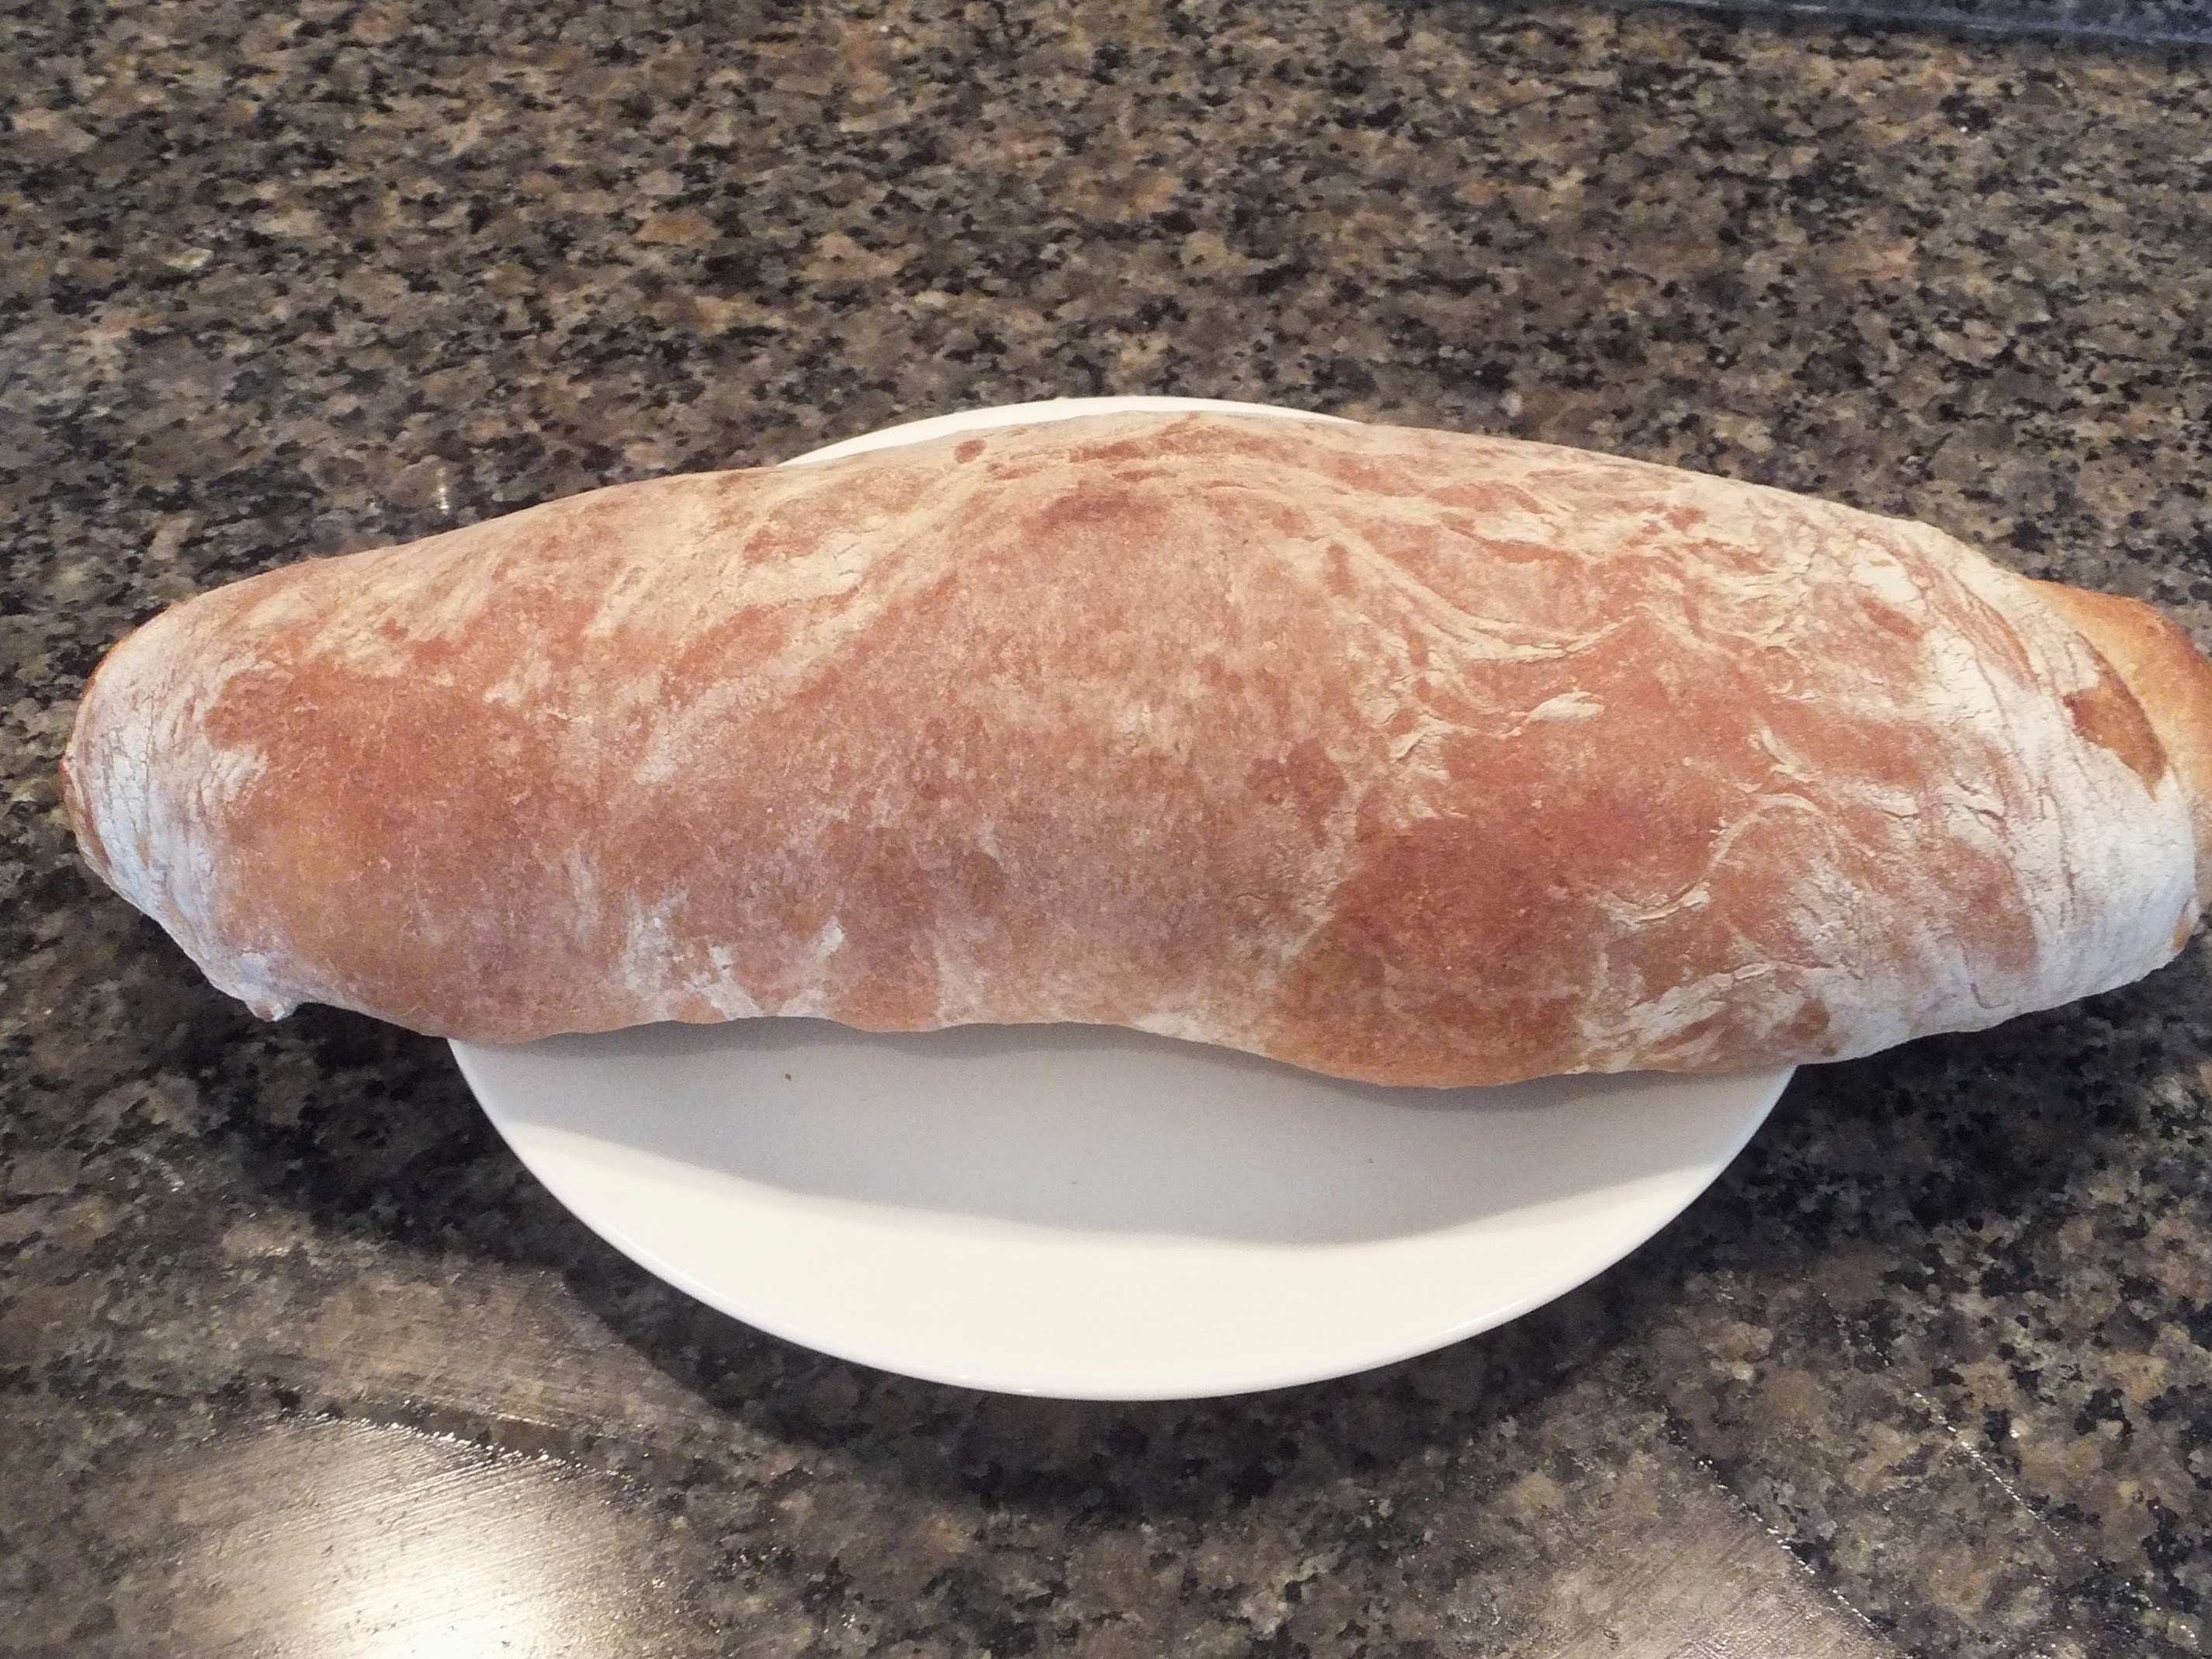
\includegraphics[width=\linewidth,trim=0px 0px 0px 0px, clip=true]{cinamon_raisin_bread-01.jpeg}
    \end{image}

    \begin{image}
      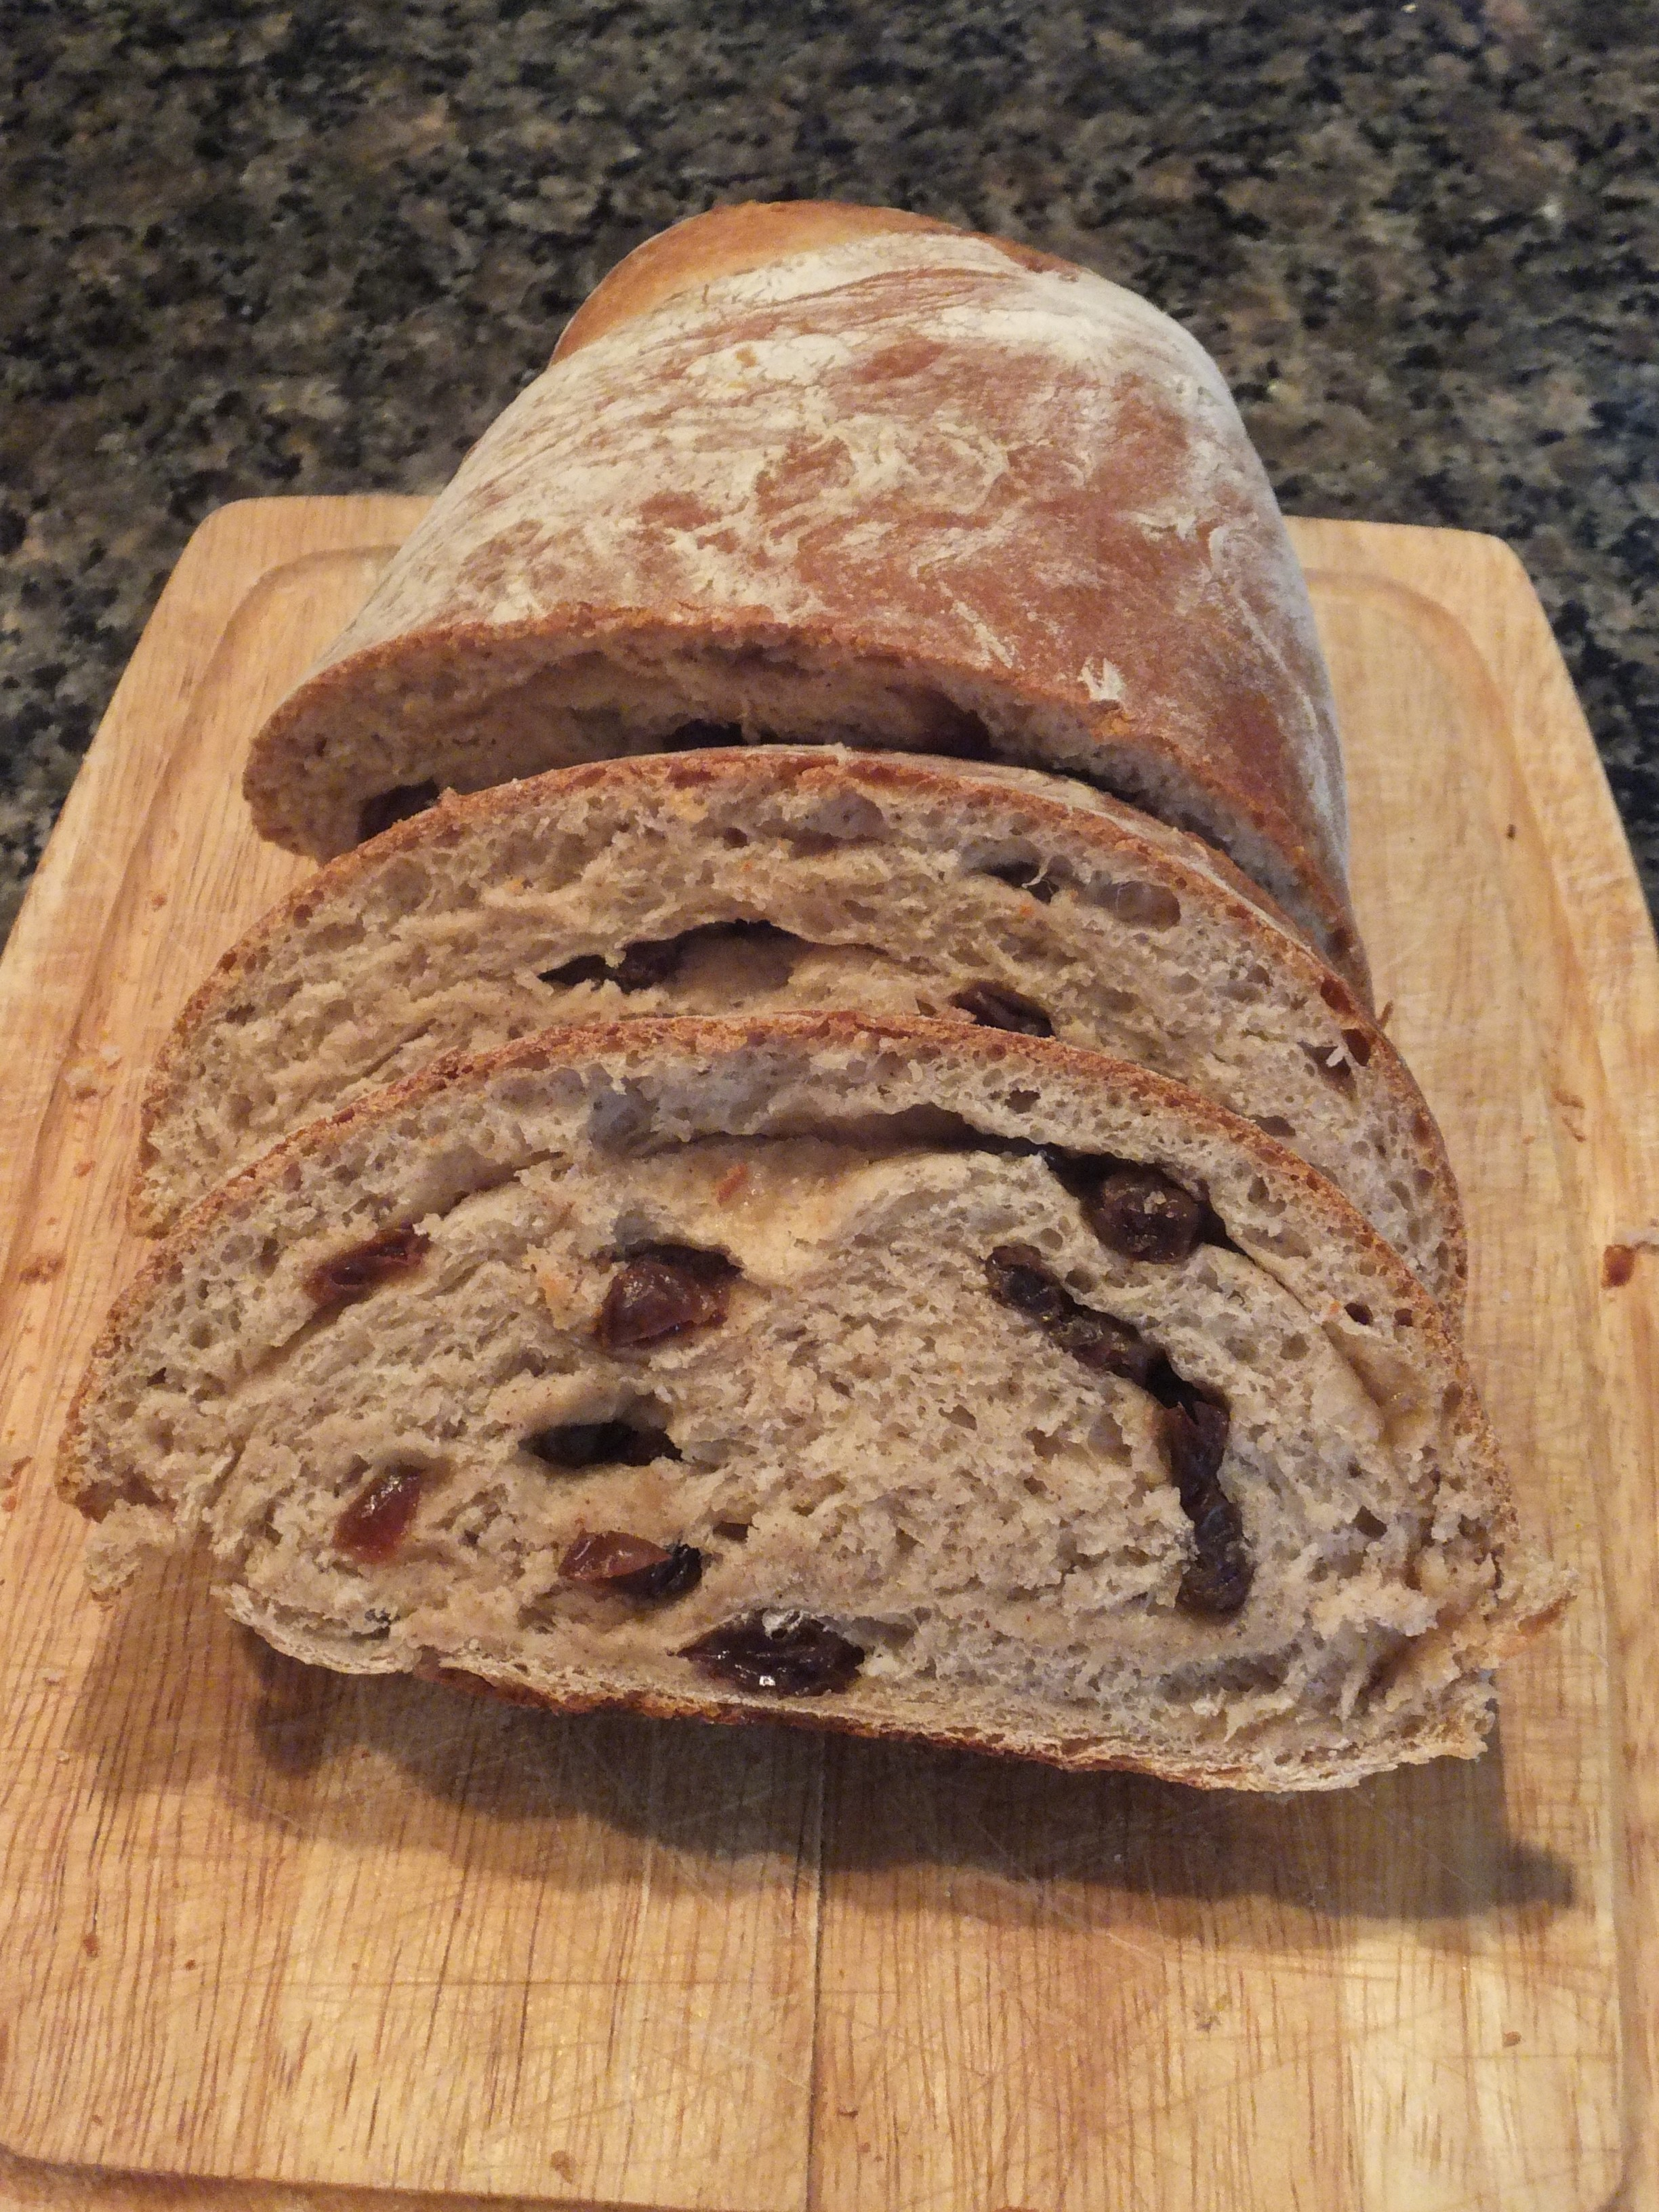
\includegraphics[width=0.75\linewidth,trim=0px 0px 0px 0px, clip=true]{cinamon_raisin_bread-02.jpeg}
    \end{image}
  \end{images}

  \begin{steps}
  \item Warm the milk and disolve 1 tbsp of the sugar and all of the
    yeast in it
  \item Cover and proof for a while
  \item Mix in the eggs, salt, and cinnamon
  \item Sift in the flour and baking powder, first whisking everything
    together, then moving to a spatula, and finally kneading it until
    everything comes together
  \item Continue kneading for 5 minutes, until the bread is smooth and
    no longer sticky
  \item Let rise in the refrigerator overnight (this will probably be
    OK out of the fridge if it's cold in your house at night)
  \item Remove the dough from the fridge and allow it to come up to
    room temperature for 2 hours
  \item Roll the dough \nicefrac{1}{4}'' thick
  \item Put the rest of the sugar, some water, and the raisins in a
    pan and heat until the raisins become soft and juicy
  \item Spread the raisins over the dough evenly
  \item Roll the bread into a loaf, making swirling patterns of
    raisins.  Use the syrup left over from the raisins to wet and seal
    the edges
  \item Allow the bread to rise for another hour in a warm place
  \item Pre-heat an oven to 400\degree F
  \item Bake the bread for 30 minutes, until brown and crusty on outside
  \item Remove the bread from the oven and invert onto a cool surface
    to prevent the bottom from burning
  \item Allow the bread to cool for minutes before cutting it,
    otherwise it won't cook through
  \end{steps}
\end{recipe}
\end{document}
